\chapter{Hypothesis Testing \& Normality}

\section{Statistical Theory}
When preforming statistical analysis, we often want to check whether or not our assumtions about data are justified. This is the realm of \emph{hypothesis testing}, where we formulate testable hypothesis about whether our data fits a given model, and then preform various statistical tests on that data to support or reject our hypothesis.

The crux of all hypothesis testing comes in the creation of two mutually exclusive outcomes for our tests. These are the \emph{null hypothesis} and the \emph{alternative hypothesis}. The null hypothesis, often written $H_0$, is a hypothesis which is ``created to be rejected'' in favor of the alternative hypothesis, $H_a$. The most common example of hypothesis testing comes in the testing of normality of our data. Here, we want to establish whether or not a normal Gaussian distribution is a reasonable parent distribution for our data. In many cases, this is a reasonable initial guess for the distribution of data, but (unsurprisingly) not all data comes from Gaussian distributions. When testing for normality, we often formulate our hypothesis as follows:
\begin{itemize}
	\item $H_0$ is the hypothesis that our data is drawn from a normal distribution.
	\item $H_a$ is the alternative, that the data was \emph{not} drawn from a normal distribution.
\end{itemize}

To provide a quantitative way to evaluate these hypothesis, we turn to the actual statistical tests. In general, statistical tests require an \emph{a priori} selection of a confidence level, denoted $\alpha$. This is a measure of ``how strict do we want our test to be?'' Lower values of $\alpha$ mean that our tests need to be ``more sure'' of their results to reject or fail to reject the null hypothesis. Closely related to the confidence level is the $p$-value; this is a measure of ``how sure our test actually is'' of our result, loosely speaking. In general, we are able to reject the null hypothesis when $p < \alpha$; this is why picking a smaller $\alpha$ makes it harder to reject $H_0$.

There are two main tests we can use to test for normality: the \emph{Shapiro-Wilk} test and the \emph{Anderson-Darling} test~[\cite{nist}]. The Shapiro-Wilk test gives a statistic\footnotetext{For the Shapiro-Wilk test, $x_{(i)}$ are the ordered sample values (in ascending magnitude), and $a_i$ are constants generated from a normal distribution with $n$ samples and the same mean and variance of the sample data.} \[ W = \frac{\qty(\sum_{i=1}^n a_ix_{(i)})^2}{\sum_{i=1}^n (x_i - \bar{x})^2}, \]
along with an associated $p$-value. The Anderson-Darling test calcualtes the statistic $A^2$, along with critical values $v_\text{crit}$ for various confidence levels. Given an $\alpha$, we choose the critical value for that confidence level and compare it to $A^2$; if $A^2 > v_\text{crit}$, we reject $H_0$, otherwise we fail to do so.

It is important to note that rejecting or failing to reject the null hypothesis are not conclusive tests for normality, or a lack thereof. Failing to reject the null hypothesis \emph{does not} imply that the alternative hypothesis is true, it merely points suggestively in that direction while winking. We also must contend with the fact that for extremely large sample sizes (on the order of tens of thousands of data points), these tests become increasingly sensitive to even minor fluctuations in the data. This can lower the validity of these test in relation to our data, so we often look for other ways to analyze the normality of data. One such method is a normal quantile plot, which divides the sample data into quantiles and plots them according to what would be expected if the data were drawn from a Gaussian. If the data is indeed normal, the quantile plot looks roughly linear.

\section{Application to SDSS Data}
\subsection*{Examining Normality with Histograms}
We'll begin by examining a histogram of $r$ band magnitude observations of quasars in the full SDSS data set.
\begin{figure}
	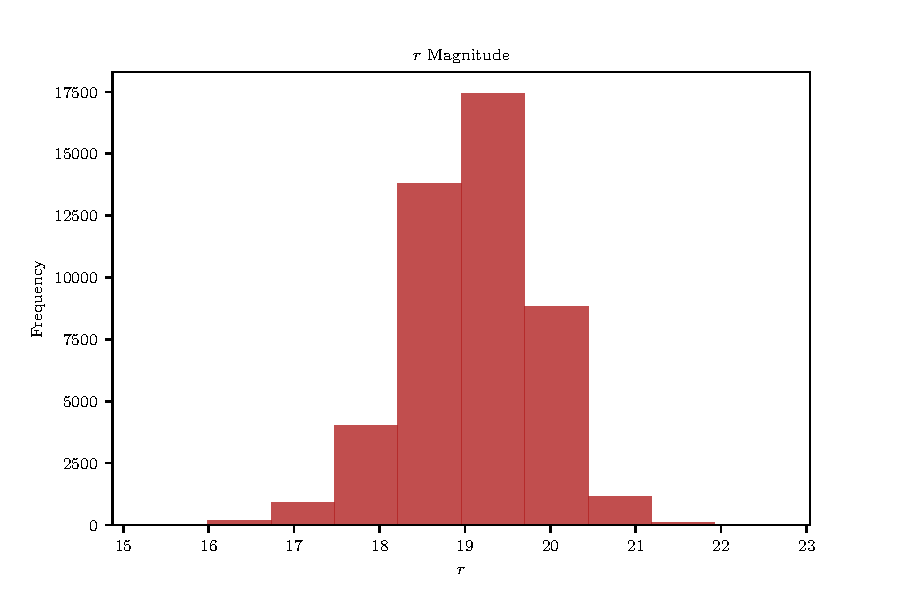
\includegraphics[width=\textwidth]{hist}
	\caption{Histogram of $r$ band magnitudes. The bin width is the default from \texttt{matplotlib}'s \texttt{hist()} function. Changing the bin width may reveal a more complicated distribution than appears in this histogram.}
\end{figure}
As we can clearly see from the graph, the $r$ band magnitude peaks somewhere between 19 and 20, and tapers off quickly to either side. From a distance, these data \emph{do} appear to be normally distributed, but the only way to get a quantitative estimate of the data's normality is to preform additional statistical tests on it. 

\subsection*{Statistical Tests for Normality}
Given that our data looks normal from a distance, we can use various tests to, well, test the normality of our data. First, we must formulate a hypothesis to test. We'll say that the null hypothesis $H_0$ is the hypothesis that our data is drawn from a Gaussian distribution. We choose an $\alpha$ of $0.01$.

First, we'll preform the Shapiro-Wilks test, to obtain a test statistic $W$ and associated $p$-value. If our $p$-value is \emph{less} than the chosen $\alpha$, we have evidence that our data is not drawn from a normal parent distribution, and we can reject $H_0$. Using \texttt{scipy.stats.shapiro()}, we obtain the following values:
\[ W \approx 0.99,\quad p \approx 0.0. \]
Since $p < \alpha$, we reject the null hypothesis under the Shapiro-Wilks test, and conclude that our data is \emph{not} normally distributed.

Next, we'll use the Anderson-Darling test to investigate normality. From this, we will obtain the test statistic $A^2$ and an associated critical value which we'll compare to investigate if the data is normally distributed. Using \texttt{scipy.stats.anderson()}, we obtain the following values:
\[ A^2 \approx 129.4, \quad v_\text{crit} = \begin{pmatrix}
	0.576 \\ 0.656 \\ 0.787 \\ 0.918 \\ 1.092
\end{pmatrix}, \]
where the critical values are for significance levels of $15\%$, $10\%$, $5\%$, $2.5\%$, and $1\%$ respectively. Since we are using $\alpha = 0.01 = 1\%$, we select the largest critical value, $v_\text{crit} = 1.092$. To analyze the results, we must compare $A^2$ to $v_\text{crit}$. Since
\[ A^2 \gg 1.092, \]
we reject $H_0$ and again conclude that our data is not normally distributed.

It is important to note that both the Shapiro-Wilks and Anderson-Darling tests suffer from the issue that for large sample sizes, the tests may detect departures from normality that are not really present in the data. Since our sample size is large (over $46,000$ data points), these results may not be conclusive in discovering departures from normality. To further investigate this, we will use a \emph{Q-Q} plot to plot theoretical quantiles against the quantiles observed in our data.
\begin{figure}
	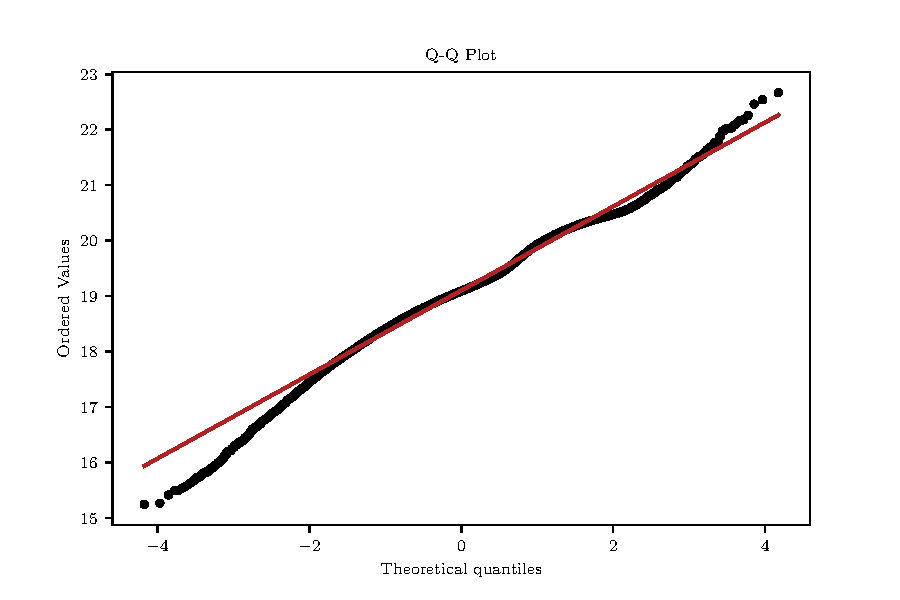
\includegraphics[width=\textwidth]{qq-plot}
	\caption{A Quantile-Quantile plot comparing theoretical quantiles of a normal distribution and the quantiles observed in the SDSS data.}
	\label{fig:qq}
\end{figure}
Observe in Figure~\ref{fig:qq} that towards the lower end of the theoretical quantiles there is significant deviation from the expected values; if the data were normally distributed, we would expect that the data points would fall on, or very near the red line. There is also slight evidence of departure from the expected quantiles towards the high-end of the plot.

\subsection*{Investigating Presence of Subpopulations}
Although our data \emph{looks} normally distributed on a histogram, every statistical test we've preformed has rejected the normality of the data. To understand why this is happening, we need to investigate what could be happening. We'll first plot the $r$ band magnitude using \emph{Scott's rule} for bin width. This will allow us to get a finer view of how our data is distributed than a normal histogram will.
\begin{figure}
	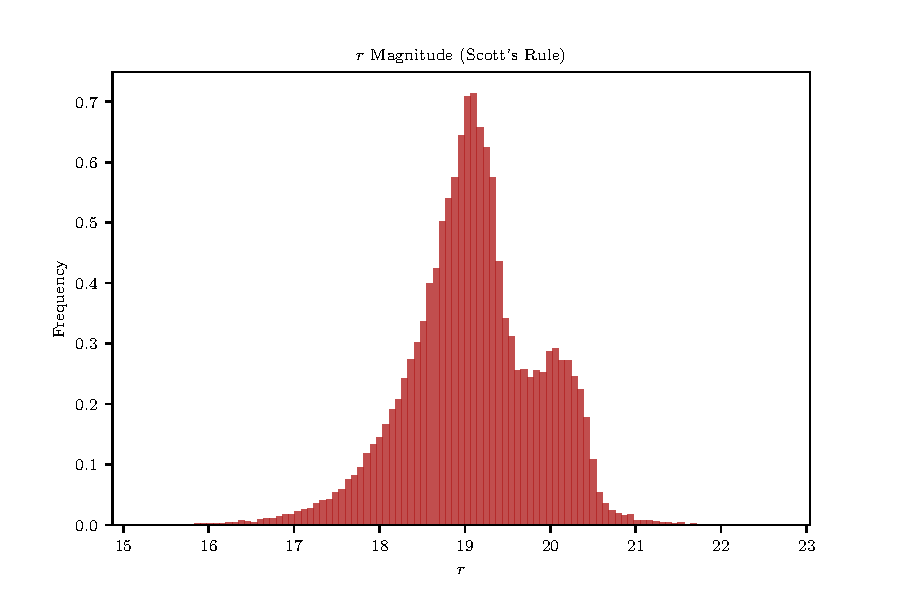
\includegraphics[width=\textwidth]{hist-scott}
	\caption{Histogram of $r$ band magnitudes, using \emph{Scott's rule} for determining bin width. Scott's rule says that the bin width $h$ should be equal to $\frac{3.5\hat{\sigma}}{n^{1/3}}$, where $\hat{\sigma}$ is the sample standard deviation and $n$ is the number of data points. In this example, $\hat{\sigma} \approx 0.76$ and $n = 46,420$.}
	\label{fig:hist-scott}
\end{figure}
Plotting the data using \emph{Scott's rule} shows us in Figure~\ref{fig:hist-scott} that our distribution appears to be bimodal, which did not show up at all on our original plot. We can investigate this apparent bimodality by looking at comparable histograms for the other passbands.
\begin{figure}
	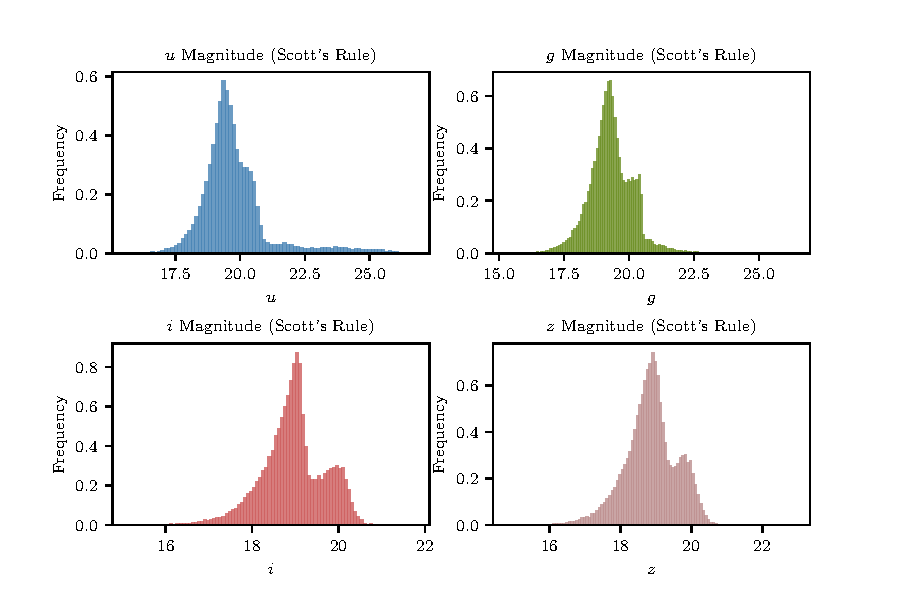
\includegraphics[width=\textwidth]{hist-colors}
	\caption{Passband magnitude histograms for the remaining color bands ($u,g,i,z$). Note the development of bimodality in the data as the color band gets progressively redder. }
	\label{fit:hist-colors}
\end{figure}

We discover that as our passbands get progressively more red, the bimodality of the brightness increases (Figure~\ref{fit:hist-colors}). When we look at brightness in the $u$ band, the data looks \emph{almost} normaly (still with significant evidence of non-normality), but in the $i$ and $z$ bands the presence of a second population of quasars is clearly visible on the histogram.